\subsection{Modulation}
\begin{enumerate}[label=\thesubsection.\arabic*.,ref=\thesubsection.\theenumi]

\numberwithin{equation}{enumi}
\numberwithin{figure}{enumi}
\numberwithin{table}{enumi}


\item See Fig. \ref{fig:ee18btech11012_fig1} for the constellation diagram.  The transmitted symbol set is given by 
\begin{align}
\vec{s}_m = \myvec{\cos \frac{2m\pi}{8}\\ \sin \frac{2m\pi}{8}}, \quad m \in \cbrak{0,1,\dots,7}.
%\textbf{y = s + n}
\end{align}
%
The numerical values for $\vec{s}_m$ are listed in Table \ref{table:ee18btech11012_fig2}
\begin{figure}[!ht]
                \resizebox{\columnwidth}{!}{\input{./ee18btech11012/figs/8psk_constellation.tex}}
\caption{Constellation diagram}
\label{fig:ee18btech11012_fig1}
\end{figure}


\item The gray code shown in Table \ref{table:ee18btech11012_fig2}
 is used for encoding the 8-PSK symbols.
\begin{table}[!ht]
                \resizebox{\columnwidth}{!}{\input{./ee18btech11012/figs/ee18btech11012_1.tex}}
\caption{Gray coding}
\label{table:ee18btech11012_fig2}
\end{table}

%$s_0$ denote bits 000, $s_1$ denote bits 001, $s_2$ denote bits 011,$s_3$ denote bits 010,$s_4$ denote bits 110,$s_5$ denote bits 111,$s_6$ denote bits 101,$s_7$ denote bits 100.

\item The received symbol is then obtained as
\begin{align}
\vec{y} = \sqrt{E_s}\vec{s} + \vec{n}
\end{align}
%
where $E_s$ is the symbol energy and 

\begin{align}
\vec{n} &\sim \mathcal{N}\brak{\vec{0},\frac{N_0}{2}\vec{I}}
\\
\vec{s} &\in \cbrak{\vec{s}_m}_{m = 0}^{7}
\end{align}

\item Using the ML criterion, the decision rule for each symbol is given by Fig. \ref{fig:ee18btech11012_fig2}.  For $\vec{s}_0$, this can be expressed as
\begin{align}
    \norm{\textbf{y}-\textbf{$s_{0}$}}^2 & \le \norm{\textbf{y}-\textbf{$s_{i}$}}^2, \quad i = 1,\dots,7\\
\implies \brak{\vec{s}_0 - \vec{s}_i}^T \vec{y} &\ge 0\\
%    \norm{\textbf{y}-\textbf{$s_{0}$}}^2 &< \norm{\textbf{y}-\textbf{$s_{1}$}}^2\\
%    \norm{\textbf{y}-\textbf{$s_{0}$}}^2 &< \norm{\textbf{y}-\textbf{$s_{2}$}}^2\\
%    \norm{\textbf{y}-\textbf{$s_{0}$}}^2 &< \norm{\textbf{y}-\textbf{$s_{3}$}}^2\\
%    \norm{\textbf{y}-\textbf{$s_{0}$}}^2 &< \norm{\textbf{y}-\textbf{$s_{4}$}}^2\\
%    \norm{\textbf{y}-\textbf{$s_{0}$}}^2 &< \norm{\textbf{y}-\textbf{$s_{5}$}}^2\\
%    \norm{\textbf{y}-\textbf{$s_{0}$}}^2 &< \norm{\textbf{y}-\textbf{$s_{6}$}}^2\\
%    \norm{\textbf{y}-\textbf{$s_{0}$}}^2 &< \norm{\textbf{y}-\textbf{$s_{7}$}}^2
\end{align}
%
which can be simplified to obtain the matrix inequality
\begin{align}
\myvec{
\brak{\vec{s}_0 - \vec{s}_1}^T \\
\brak{\vec{s}_0 - \vec{s}_2}^T\\
\brak{\vec{s}_0 - \vec{s}_3}^T\\
\brak{\vec{s}_0 - \vec{s}_4}^T\\
\brak{\vec{s}_0 - \vec{s}_5}^T\\
\brak{\vec{s}_0 - \vec{s}_6}^T\\
\brak{\vec{s}_0 - \vec{s}_7}^T
}\vec{y} \succeq \vec{0} 
%    (s_{0}-s_{1})^Ty>0
%    (s_{0}-s_{2})^Ty>0
%    (s_{0}-s_{3})^Ty>0
%    (s_{0}-s_{4})^Ty>0
%    (s_{0}-s_{5})^Ty>0
%    (s_{0}-s_{6})^Ty>0
%    (s_{0}-s_{7})^Ty>0
\end{align}
%
resulting in 
\begin{align}
\myvec{\sqrt{2} - 1 & 1 \\ \sqrt{2} - 1 & -1} \vec{y} \succeq \vec{0}
\end{align}

\begin{figure}[!ht]

                \resizebox{\columnwidth}{!}{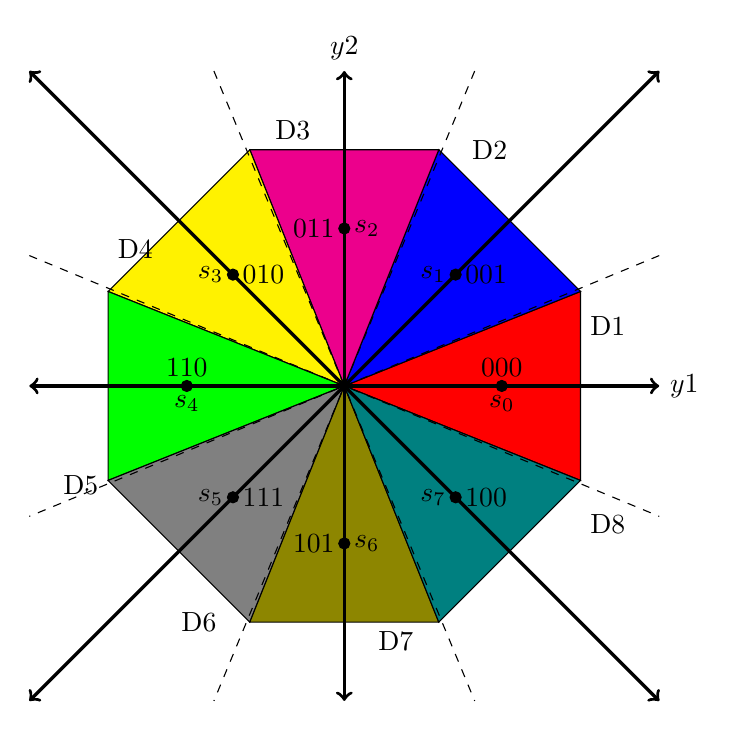
\begin{tikzpicture}
\draw[fill=red]  (0,0) -- (3,1.2) -- (3,-1.2) -- (0,0) -- cycle;
\draw[fill=blue]  (0,0) -- (1.2,3) -- (3,1.2) -- (0,0) -- cycle;
\draw[fill=magenta!100]  (0,0) -- (-1.2,3) -- (1.2,3) -- (0,0) -- cycle;
\draw[fill=yellow]  (0,0) -- (-1.2,3) -- (-3,1.2) -- (0,0) -- cycle;
\draw[fill=green]  (0,0) -- (-3,1.2) -- (-3,-1.2) -- (0,0) -- cycle;
\draw[fill=gray]  (0,0) -- (-3,-1.2) -- (-1.2,-3) -- (0,0) -- cycle;
\draw[fill=olive]  (0,0) -- (-1.2,-3) -- (1.2,-3) -- (0,0) -- cycle;
\draw[fill=teal]  (0,0) -- (1.2,-3) -- (3,-1.2) -- (0,0) -- cycle;
\draw[<->,very thick] (-4,0)--(4,0) node[right]{$y1$};
\draw[<->,very thick] (0,-4)--(0,4) node[above]{$y2$};
\draw[dashed] (4,1.656)--(-4,-1.656);
\draw[dashed] (1.656,4)--(-1.656,-4);
\draw[dashed] (-1.656,4)--(1.656,-4);
\draw[dashed] (-4,1.656)--(4,-1.656);
\draw[<->,very thick](-4,-4)--(4,4);
\draw[<->,very thick](-4,4)--(4,-4);

\filldraw[black] (2,0) circle (2pt) node[below] {$s_0$} node[above] {000};
\filldraw[black] (1.414,1.414) circle (2pt) node[left] {$s_1$} node[right] {001};
\filldraw[black] (0,2) circle (2pt) node[right] {$s_2$} node[left] {011};
\filldraw[black] (-1.414,1.414) circle (2pt) node[left] {$s_3$} node [right] {010};
\filldraw[black] (-2,0) circle (2pt) node[below] {$s_4$} node[above] {110};
\filldraw[black] (-1.414,-1.414) circle (2pt) node[left] {$s_5$} node[right] {111};
\filldraw[black] (0,-2) circle (2pt) node[right] {$s_6$} node[left] {101};
\filldraw[black] (1.414,-1.414) circle (2pt) node[left] {$s_7$} node [right] {100};

\foreach \coordinate/\label/\pos in {{(3,1)/D1/below right},{(1.5,3)/D2/right},{(-1,3)/D3/above right},{(-3,1.5)/D4/above right},{(-3,-1.5)/D5/above left},{(-1.5,-3)/D6/left},{(1,-3)/D7/below left},{(3,-2)/D8/above right}} \node[\pos] at \coordinate {\label};

\end{tikzpicture}
}

\caption{decision regions}
\label{fig:ee18btech11012_fig2}
	
\end{figure}

%\begin{figure}[!ht]
%
%                \resizebox{\columnwidth}{!}{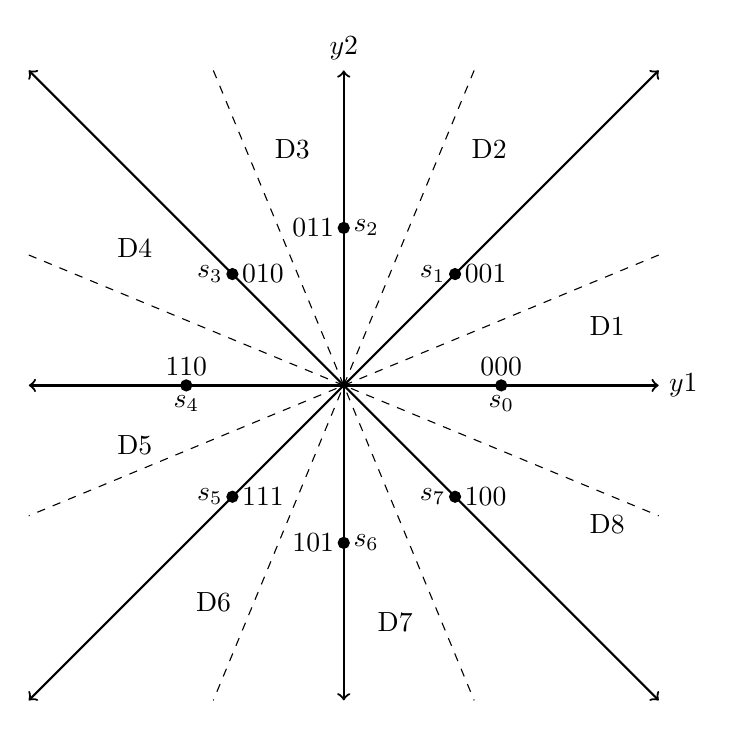
\begin{tikzpicture}

\draw[<->,thick] (-4,0)--(4,0) node[right]{$y1$};
\draw[<->,thick] (0,-4)--(0,4) node[above]{$y2$};
\draw[dashed] (4,1.656)--(-4,-1.656);
\draw[dashed] (1.656,4)--(-1.656,-4);
\draw[dashed] (-1.656,4)--(1.656,-4);
\draw[dashed] (-4,1.656)--(4,-1.656);
\draw[<->,thick](-4,-4)--(4,4);
\draw[<->,thick](-4,4)--(4,-4);

\filldraw[black] (2,0) circle (2pt) node[below] {$s_0$} node[above] {000};
\filldraw[black] (1.414,1.414) circle (2pt) node[left] {$s_1$} node[right] {001};
\filldraw[black] (0,2) circle (2pt) node[right] {$s_2$} node[left] {011};
\filldraw[black] (-1.414,1.414) circle (2pt) node[left] {$s_3$} node [right] {010};
\filldraw[black] (-2,0) circle (2pt) node[below] {$s_4$} node[above] {110};
\filldraw[black] (-1.414,-1.414) circle (2pt) node[left] {$s_5$} node[right] {111};
\filldraw[black] (0,-2) circle (2pt) node[right] {$s_6$} node[left] {101};
\filldraw[black] (1.414,-1.414) circle (2pt) node[left] {$s_7$} node [right] {100};

\foreach \coordinate/\label/\pos in {{(3,1)/D1/below right},{(1.5,3)/D2/right},{(-1,3)/D3/right},{(-3,1.5)/D4/above right},{(-3,-1)/D5/above right},{(-2,-3)/D6/above right},{(1,-3)/D7/left},{(3,-2)/D8/above right}} \node[\pos] at \coordinate {\label};

\end{tikzpicture}
}
%
%\label{fig:ee18btech11012_fig2}
%\caption{decision regions}
%	
%\end{figure}



Similarly the decisions for all symbols 
are available in Table \ref{table:ee18btech11012_fig4}
%
\begin{table}[!ht]
%                \resizebox{\columnwidth}{!}{\input{./ee18btech11012/figs/ee18btech11012_2_new.tex}}
                \resizebox{\columnwidth}{!}{\input{./ee18btech11012/figs/ee18btech11012_2.tex}}
\caption{Decision regions and their inequalities}
\label{table:ee18btech11012_fig4}
\end{table}



\end{enumerate}
